% Created 2023-10-31 火 01:38
% Intended LaTeX compiler: pdflatex
\documentclass[dvipdfmx,11pat]{jarticle}
\usepackage[utf8]{inputenc}
\usepackage[T1]{fontenc}
\usepackage{graphicx}
\usepackage{longtable}
\usepackage{wrapfig}
\usepackage{rotating}
\usepackage[normalem]{ulem}
\usepackage{amsmath}
\usepackage{amssymb}
\usepackage{capt-of}
\usepackage{hyperref}
\setlength{\textwidth}{18cm}
\setlength{\oddsidemargin}{-1cm}
\setlength{\evensidemargin}{-1cm}
\setlength{\topmargin}{-2cm}
\setlength{\textheight}{26cm}
\author{鈴木正幸,岩手大学・非常勤講師 suzuki@iwate-u.ac.jp}
\date{\today}
\title{コンピュータと数式処理}
\begin{document}

\maketitle
URL: \url{https://github.com/masayuki054/comp\_and\_cal/}


\section{数理科学研究のための情報計算リテラシ}
\label{sec:org7cf90d8}
情報計算リテラシという言葉で,コンピュータやインターネットを用いた,情
報や文書の読み書き共有,多大なデータの計算や表示など,を行なう際の,考
え方とツールの使い方を意味することにします。

本講では,理工学研究分野での情報計算リテラシとして,
大きく次の3点についてお話しします。

\begin{itemize}
\item 数理科学的に考えること書くことを支援するデジタルツールについて,思考
法などを含めてお話しします。

\item 数理科学的な計算道具については,計算科学とは何か,どんなプログラムが
あるのかについてお話しします。特に,重要な,偏微分方程式を解くための
有限要素法を例にお話しします。数式処理との関連についても。

\item 計算,検索,探索,数理とはについて考えるために,数式処理における重要
なアルゴリズムである,グレブナー基底計算と多変数代数方程式の解法につ
いて概観します。
\end{itemize}

\section{私的研究興味の内容 \url{./interests.org} 参照}
\label{sec:org9413581}

\section{研究のための情報リテラシー}
\label{sec:org1d1e416}

\href{https://masayuki054.github.io/ict\_literacy\_for\_thinking\_and\_memo/}{
メモと思考のためのICTの活用}

\href{https://masayuki054.github.io/cloud\_and\_information\_literacy/talk.html}{クラウドと情報リテラシー}

\begin{itemize}
\item 思考し実験し記録し理解し文書を作成するためのリテラシ
\item 基本技術は思考法, 文書作成も思考法
\item 思考は情報処理プロセス
\end{itemize}

\subsection{知的思考の技術}
\label{sec:org982108e}
\begin{itemize}
\item 思考過程の見える化
\item 発想法,水平思考,放射思考
\item 論理的思考法,批判的思考
\end{itemize}

\subsection{プロセス管理法}
\label{sec:org1ae8332}
\begin{itemize}
\item 計算論的思考
\item GTD (Getting Things Done)
\item ストレスフリー
\end{itemize}

\subsection{思考のためのデジタルツール}
\label{sec:org36ed512}
考えることをサポートするデジタルツールがある

\subsubsection{考える,記憶する,こととは?}
\label{sec:orgd84e836}

\begin{itemize}
\item 思考の基本 抽象化と詳細化 , So What, Why so, MECE
\item 思考の記録 MECE, 構造化,GTD
\end{itemize}

\begin{enumerate}
\item いろいろな思考法
\label{sec:orgcabe438}
\begin{itemize}
\item 論理的思考
\item 批判的思考
\item 発想法
\item 水平思考
\item 計算論的思考
\end{itemize}

\item 知的思考の技術
\label{sec:orgc0b6600}
\begin{itemize}
\item 思考の見える化
目的探索,観察,発想,分類,構造化,意志決定,表現
\end{itemize}
\end{enumerate}

\subsubsection{情報リテラシーは思考法である}
\label{sec:org562a511}
\begin{itemize}
\item 生のデータを意味付けして情報になる
\item 知的情報リテラシーの技術
\begin{itemize}
\item 情報の収集,加工,分析,蓄積,生成
\end{itemize}
\end{itemize}

\subsubsection{理解の記録(外化,メモや文書)}
\label{sec:org09bc5e1}
\begin{itemize}
\item 理解を外化する. 小さな理解のくりかえしを,構造的に記録する
\item 内化しやすい外化
\begin{itemize}
\item 論理的に理解しやすい外化はアウトライン構造
\item イメージしやすい外化は,マインドマップ構造
\end{itemize}
\item 外化の意味付
\begin{itemize}
\item 情報を外に出すことは二つの意味がある
\begin{itemize}
\item 内的情報を外部記憶に置くこと
こっちが外化, これがメモ
\item 自分の情報を他者が理解できる形にすること
第三者への情報 客観化,文書化
\end{itemize}
\end{itemize}

\item 理解と知識と外化
\begin{itemize}
\item 小さな理解と大きな理解,整合性の問題
\item 理解の再帰性
\end{itemize}
\end{itemize}

\begin{enumerate}
\item コンピュータとインターネットの意味
\label{sec:org9770713}
思考と記憶を補助し,外化を促すこと
\begin{itemize}
\item 情報を保存し共有すること
\item 検索できるようにすること
\item 人と計算機の共同作業の実現,互いに補完と拡張
\end{itemize}
\end{enumerate}

\section{計算リテラシ}
\label{sec:orgd5a0748}
\begin{itemize}
\item 計算科学と数学ソフトウェア
\item プログラミングによる計算プロセス管理
\item 計算のための数学
\begin{itemize}
\item 微分から差分へ
\item 方程式の解法,連立一次方程式
\end{itemize}
\end{itemize}

\subsection{計算科学とは}
\label{sec:orge121d5e}

\href{https://ja.wikipedia.org/wiki/\%E8\%A8\%88\%E7\%AE\%97\%E7\%A7\%91\%E5\%AD\%A6}{計算科学 - Wikipedia} とは

数学的モデルとその定量的評価により、計算機を用いて問題を解決する
様々な問題の計算機によるシミュレーションやその他の計算手法の適用を指す。


数値解析は,数式ではなく,実際の数を対象とし,物理現象など現実の対象をモデル化した
ものである。

対象領域をモデル化したプログラムやアプリケーションソフトウェアを開発し、
それに様々なパラメータを与えて実行する。

\subsubsection{数値解析}
\label{sec:org695356b}
\begin{itemize}
\item 精度保証付き数値計算
\item 数値線形代数
\item 常微分方程式の数値解法、偏微分方程式の数値解法、数値積分
\end{itemize}

\subsubsection{数値シミュレーション}
\label{sec:org34994b3}
\begin{enumerate}
\item 目的
\label{sec:orga8ef877}
\begin{itemize}
\item 既知の事象を再構築して理解する(例えば、地震、津波などの自然災害)。
\item 既知のシナリオを最適化する(例えば、工学的プロセスや産業プロセス)。
\item 未来または未知の状況を予測する(例えば、気象、原子レベル以下の粒子の振る舞い)。
\item 気象、飛行機の周辺の気流、自動車衝突時の車体の状況、銀河系の星々の動き、爆発物など
\end{itemize}

\item 数値シミュレーションプログラムの実行
\label{sec:org007f8f2}
\begin{itemize}
\item コンピュータのメモリ内に論理的メッシュ(網目)を形成し、個々の領域が実世界
のモデルの空間的な一部分を表すようになっている。
\item 気象の場合、ひとつの点が数キロ平方の領域に対応し、その下の地
理状態、風向き、湿度、温度、気圧といったパラメータが与えられる。
\item プログラムはシミュレートする時間間隔に従って、現在の状態を基に次の状
態を計算する。
\item この計算はモデル化された方程式を解くことで行われる。そのような計算を
次々に行っていくのである。
\end{itemize}
\end{enumerate}

\subsubsection{科学的方法}
\label{sec:org66077bf}
計算科学は科学の第三の形態で、実験/観測と理論の間を補間するもの、とい
う主張もある。

\subsubsection{有限要素法(FEM)}
\label{sec:orgcefe65b}
偏微分方程式ソルバ (PDE)の 最も一般的な数値的解法

\begin{itemize}
\item 有限要素法 (FEM)とは、偏微分方程式 (PDE)の定義域 (W)の近似解を
求めるときに使用する数値的解法です。PDEを解くときの最大の難関は、解
を近似的に表す基底関数を作る工程です。基底関数の作り方は数多くありま
すが、どれを使用するかは選択した定式化によって決まります。

\item 線形 / 非線形 / 座屈 / 熱 / 動的 / 疲労解析で使用できます。
\end{itemize}

\subsection{数学ソフトウェア}
\label{sec:org3daffb0}
\subsubsection{MathLibre  \href{https://www.geogebra.org/m/hShSTr6e}{KNOPPIX/Math->MathLibre}}
\label{sec:org51cb082}
\begin{itemize}
\item DVD起動Linuxで,

\item オープン・ソースで,

\item フリーな数学ソフトウェアを収録 

\href{https://www.geogebra.org/m/hShSTr6e}{数学ソフトウェア紹介 - GeoGebraBook}
\end{itemize}

\begin{enumerate}
\item \href{https://ja.wikipedia.org/wiki/\%E6\%95\%B0\%E5\%AD\%A6\%E3\%82\%BD\%E3\%83\%95\%E3\%83\%88\%E3\%82\%A6\%E3\%82\%A7\%E3\%82\%A2}{数学ソフトウェアとは - Wikipedia}
\label{sec:org60ba49a}

\begin{enumerate}
\item ソフトウェア電卓  

\href{http://ja.numberempire.com/}{数の帝国 - 数学ツール} 数の帝国は、強力な数学ツールと数について
の知識のコレクションです。

\item 数式処理システム

\begin{itemize}
\item \href{https://ja.wikipedia.org/wiki/Sage\_(\%E6\%95\%B0\%E5\%BC\%8F\%E5\%87\%A6\%E7\%90\%86\%E3\%82\%B7\%E3\%82\%B9\%E3\%83\%86\%E3\%83\%A0)}{Sage (数式処理システム) - Wikipedia}

\item \href{http://www.wolframalpha.com/}{Wolfram|Alpha: Computational Knowledge Engine}
\end{itemize}

\item 数値解析
\begin{itemize}
\item \href{https://matome.naver.jp/odai/2136163231573327601}{MATLABの代わりに使えるソフトウェアまとめ- NAVER まとめ}
\item \href{http://signalprocessor.blogspot.jp/2016/}{信号処理のお仕事メモ: 2016} (Octave)
\item \href{http://www.inaba-lab.org/wiki/index.php/Octave\%E5\%85\%A5\%E9\%96\%80}{Octave入門 - 東海大学 コンピュータ応用工学科 稲葉研究室Wiki}
\end{itemize}
\end{enumerate}
\end{enumerate}

\subsubsection{\href{http://www.sagemath.org}{Sage} とは}
\label{sec:orgd73b297}

\href{http://www.gregorybard.com/Sage.html}{Gregory V. Bard} 曰く

\begin{itemize}
\item フリーでオープン・ソースで,
\item Maple, Mathematica, Magma, and Matlab に並らぶ,
\item 数学科の学生に最適な
\item 「コンピュータ代数」システム
\end{itemize}

\begin{enumerate}
\item Sage on the Web(1)
\label{sec:org6374767}

\begin{itemize}
\item Webで動く,
\item ノートやデスクトップPCへのインストールは必要ない。
\end{itemize}

\begin{enumerate}
\item クラウド・サーバ
\label{sec:org09718de}

\href{http://www.cocalc.com/}{CoCalc.com Sage クラウド・サーバ} 

\begin{itemize}
\item 長めの問題向き,
\item プログラムの保存ができる
\item 登録とログインが必要,
\end{itemize}

\item セル・サーバ
\label{sec:orgbb2746e}

\href{http://sagecell.sagemath.org/}{SageMathCell Server}

\begin{itemize}
\item 短かめの問題向き

\item \href{http://www.gregorybard.com/videos/Sage\_part1.swf}{関数,微分,積分,2次元プロット} の例題動画

\item \href{http://www.gregorybard.com/videos/Sage\_part2.swf}{因数分解,3次元プロット}
\end{itemize}

\item 例題
\label{sec:orgfc665bd}
\begin{verbatim}
x,y = var('x y')
plot3d(sin(x+y), [x,-pi,pi], [y, -pi, pi])
\end{verbatim}

\begin{verbatim}
Launched jmol viewer for Graphics3d Object
\end{verbatim}
\end{enumerate}


\item Sagemath アプリ
\label{sec:org7193175}

数式処理が,スマホで動くなんて,ほんとにビックリ

\begin{itemize}
\item \href{https://itunes.apple.com/jp/app/sage-math/id496492945?mt=8}{Sage Mathを App Store で}

\item \href{https://play.google.com/store/apps/details?id=org.sagemath.droid\&hl=ja}{Sage Math - Google Play の Android アプリ}
\end{itemize}

\item 入門
\label{sec:org5684bc5}

\begin{itemize}
\item \href{http://doc.sagemath.org/html/ja/tutorial/index.html}{Sageチュートリアル.ja} すぐ後で,実行しながら,説明します

\item \href{http://doc.sagemath.org/pdf/ja/tutorial/tutorial-jp.pdf}{Sage tutorial-jp.pdf}

\item \href{http://www.pwv.co.jp/\%7Etake/TakeWiki/index.php?sage\%2Fsage\%E3\%81\%AE\%E7\%B4\%B9\%E4\%BB\%8B}{sage/sageの紹介 - PukiWiki} たけもとさん

\begin{itemize}
\item \href{http://www.pwv.co.jp/\~take/TakeWiki/index.php?sage\%2F\%E8\%A8\%88\%E7\%AE\%97\%E3\%81\%97\%E3\%81\%A6\%E3\%81\%BF\%E3\%82\%88\%E3\%81\%86}{sage/計算してみよう - PukiWiki}
\end{itemize}

\item \href{http://www.sagemath.org/help-video.html}{series of videos/screencasts}
\end{itemize}

\item 例題
\label{sec:org5a2e009}

\begin{itemize}
\item \href{http://doc.sagemath.org/html/en/constructions/index.html}{プログラムの制作例}
\begin{itemize}
\item いろいろな例題と解答
\end{itemize}

\item \href{https://wiki.sagemath.org/interact}{対話的なデモリポジトリ} 
\begin{itemize}
\item interact / calculus / Taylor  を見てみよう
\end{itemize}
\end{itemize}

\item Sagemath に関する本 (フリー)
\label{sec:org6564e08}

\begin{itemize}
\item \href{http://www.gregorybard.com/Sage.html}{Sage for undergraduates, free pdf}   このページ内に pdf へのリンクが

\item \href{http://mosullivan.sdsu.edu/Teaching/sdsu-sage-tutorial/index.html}{Welcome to the SDSU Sage Tutorial}
\end{itemize}

\item Sagemath に関するいろいろなページ
\label{sec:orgd41b4fc}

\href{http://sk.sagepub.com/reference}{SAGE Knowledge - Reference} reference の検索

\href{https://qiita.com/HirofumiYashima/items/6bb5770961a3b7d33118}{Sageに関するリンク集}

\href{http://wiki.sagemath.org/quickref}{large collection of quick-reference cards} 

\url{http://sagemath.org} \url{http://doc.sagemath.org} 

\item Octave との連携
\label{sec:org0ac7f7c}

\href{http://www.pwv.co.jp/\%7Etake/TakeWiki/index.php?sage\%2FSage\%E3\%81\%A7Octave\%E3\%82\%92\%E4\%BD\%BF\%E3\%81\%86}{sage/SageでOctaveを使う - PukiWiki} 

\href{http://www.inaba-lab.org/wiki/index.php/Octave\%E5\%85\%A5\%E9\%96\%80}{Octave入門 - 東海大学 コンピュータ応用工学科 稲葉研究室Wiki}

\item \LaTeX{}とSage
\label{sec:org886851c}

\begin{itemize}
\item オンライン\LaTeX{}サービス  \href{https://oku.edu.mie-u.ac.jp/\~okumura/texonweb/}{\TeX{} を使ってみよう}

\item \href{https://mytexpert.osdn.jp/index.php?LaTeX\%A4\%CB\%A4\%E8\%A4\%EB\%CF\%C0\%CA\%B8\%BA\%EE\%C0\%AE\%A4\%CE\%BC\%EA\%B0\%FA\%A4\%AD}{\LaTeX{}による論文作成の手引き - MyTeXpert}

\item \href{http://sage.math.gordon.edu/home/pub/51/}{Using \LaTeX{} in Sage -- Sage}
\end{itemize}
\end{enumerate}

\subsection{数式処理アルゴリズム}
\label{sec:orgeb14482}

\subsubsection{不定積分入門}
\label{sec:org537d994}
\href{http://www-sop.inria.fr/cafe/Manuel.Bronstein/publications/issac98.pdf}{symbolic integration tutorial--issac98.pdf}
wikipedia の参考文献にあった

\subsubsection{規則と簡約化と検索のための計算機代数}
\label{sec:org69094e8}

高次多変数代数方程式の解法として別途,資料\url{./gbasis/gbasis.org}を配
布します。

グレブナー基底に関する用語とブッフバーガー算法については,\href{https://ja.wikipedia.org/wiki/\%E3\%82\%B0\%E3\%83\%AC\%E3\%83\%96\%E3\%83\%8A\%E3\%83\%BC\%E5\%9F\%BA\%E5\%BA\%95}{グレブナー基底 - Wikipedia} 
を参照します。

数学と検索と簡約のつながりについて,考えます。人は理論を考え,コン
ピュータに検索してもらいましょう。

多くの変数の高い次数の方程式の解法を,線形代数の概念に翻訳し,線形空間
の概念と計算に帰着します。見通しと効率が良くなります。


\section{まとめ}
\label{sec:orge7d6845}
本講では,理工学研究分野での情報計算リテラシとして,
以下の点についてお話ししたつもりです:

\begin{itemize}
\item 思考について紹介し,知的思考の7つのステップ,
わかるとはどういうことか,が重要だと考えます。

\item 思考法について,論理的思考,批判的思考,発想,抽象化と詳細化,
を紹介し,それらを支援してくれる,デジタルツール,マインドマップとア
ウトライナーを紹介しました。

\item 計算科学のためのフリーソフトウェアについて,どんな分野がありどんなア
プリがあるかについて紹介しました。

\item 数値解析において,微分と線形代数の意味を理解することが非常に大事であること

\item 代数的計算を行ってくれる言語とシステムがあること

\item 代数的アルゴリズムの例として,グレブナー基底計算と多変数代数方程式の解法について概観しました。
\begin{itemize}
\item 多項式のイデアルを,頭項,項順序,簡約規則により,構造化することで,
\item イデアルの要素を0に簡約できるグレブナー基底が計算できる
\item その意味付けにおいて線形代数が有効であり,
\item 正規形,順序,置き換え規則の完備化により,無限集合の中の検索を,
有限集合の中での簡約で計算できる
\item ユークリッドの互除法,ガウスの消去法,グレブナー基底による簡約の間
に共通な考え方が存在する
\end{itemize}
\end{itemize}

\begin{center}
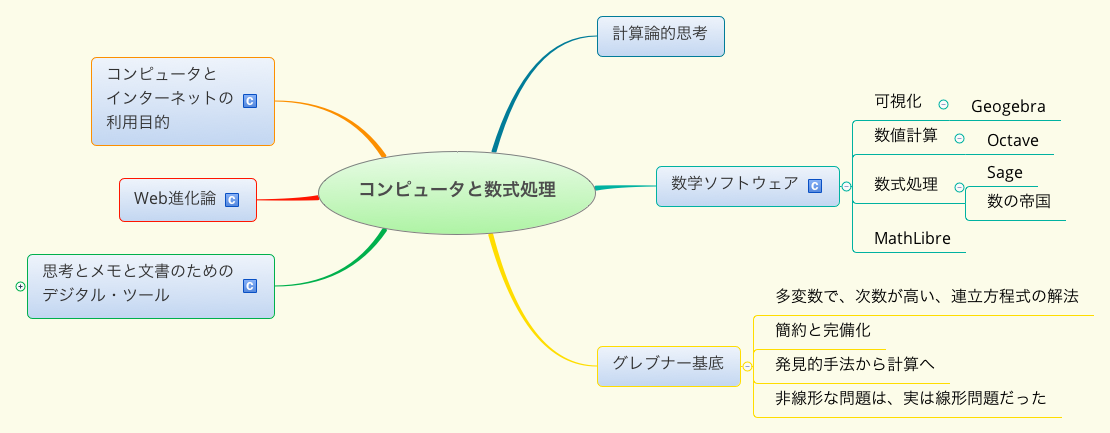
\includegraphics[width=18cm]{./map-images/01-computer_and_cal.png}
\end{center}

\begin{figure}[htbp]
\centering
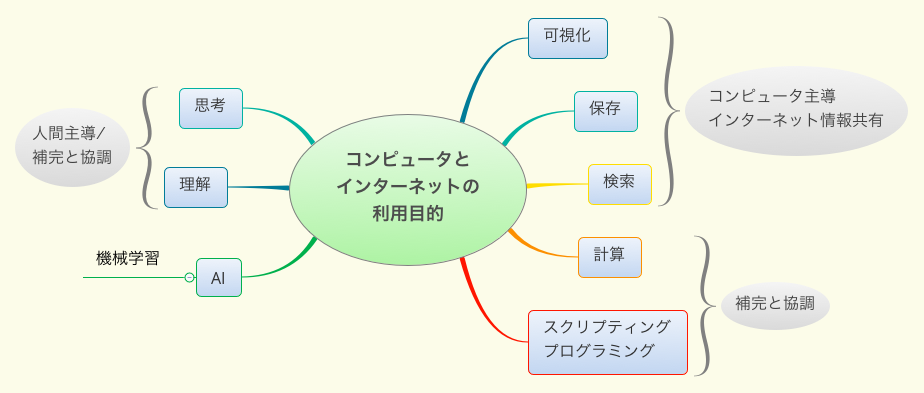
\includegraphics[width=18cm]{./map-images/03-how_to_use_computer_and_internet.png}
\caption{人とコンピュータとインターネット}
\end{figure}


\vspace{3cm}

\begin{figure}[htbp]
\centering
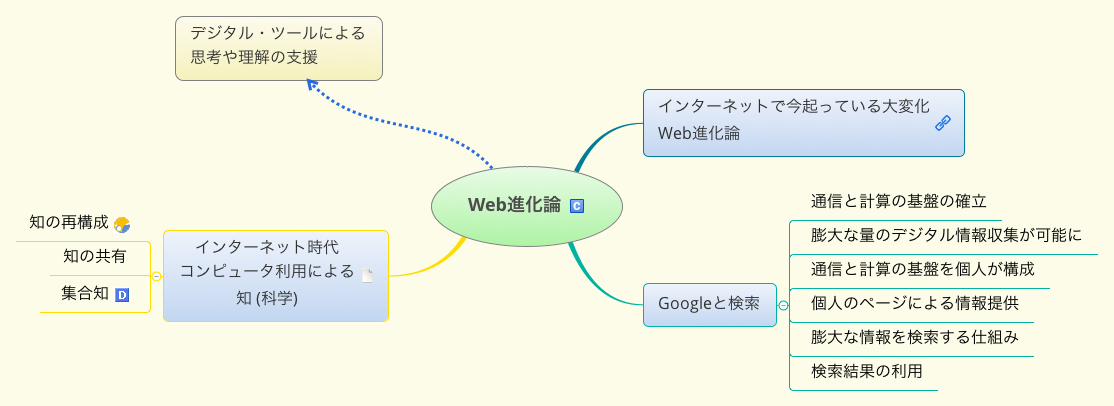
\includegraphics[width=18cm]{./map-images/04-Web_revolution.png}
\caption{インターネットが起している変革}
\end{figure}


\begin{figure}[htbp]
\centering
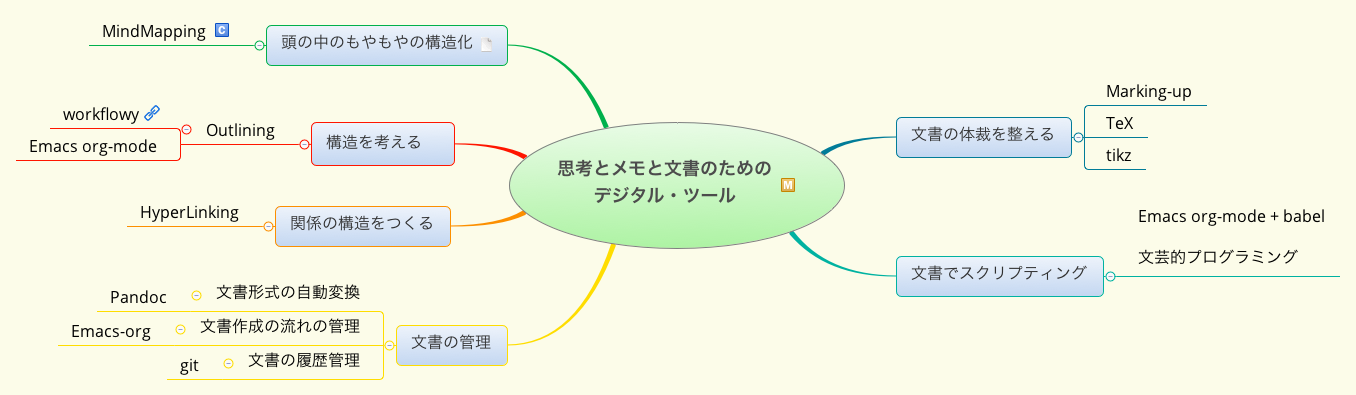
\includegraphics[width=18cm]{./map-images/05-digital_tools_for_thinking.png}
\caption{思考とメモと文書のためのデジタル・ツール}
\end{figure}
\end{document}